% Chapter Template

\chapter{Introduction} 
\label{chapter-introduction} 

%----------------------------------------------------------------------------------------
%	SECTION 
%----------------------------------------------------------------------------------------

\section{Motivation}

In recent years, tremendous progress has been made in the field of Artificial Intelligence (AI), especially in Deep Learning \citep{lecun-dl, deeplearning-overview}. Deep Learning has helped AI systems reach and sometimes surpass human-level perception, mainly in computer vision \citep{image-recognition} and natural language processing \citep{machine-translation}. This has given rise to amazing industrial applications such as autonomous driving, early cancer detection, enhanced machine translation, etc. In safety-critical contexts, a key concern of engineers is to make sure the trained models are error-free, which can be challenging if the input data does not hold sufficient information to reduce the uncertainty on the predictions to an admissible level.

One possible solution researchers have been exploring is to use multiple modalities\footnote{The term modality, also called mode, is generally understood to mean "the way in which something happened or is experienced" \citep{taxomany-multimodal}}, which has largely been inspired by the often multi-modal nature of information gathering processes in humans, i.e., we see objects, hear sound, feel the texture, smell odours, and taste flavours. Multi-modal deep learning (MMDL) essentially consists in exploiting information from different channels and in different forms in the hope that the information carried by each mode is (partially) complementary, in order to improve the predictive performance of deep learning models. For example, in \citep{lidar-camera} sensorial inputs from wide-angle cameras and LIDAR\footnote{Laser Detection and Ranging} sensors are combined for road detection. Cameras provide dense information over a long range under good illumination conditions and fair weather, whereas LIDARs are only marginally affected by the external lighting conditions but have a limited range. Thus, merging the complementary information of the two sensors improves the accuracy of the road detection process. Despite its improvements on the predictions, MMDL still suffers from a major drawback. Indeed, no systematic mechanisms exist to handle failing modes. In the present report, a mode is said to be failing if a) it has a high noise to signal ratio, b) the data is much different from the training data, c) the data is missing. Failing modes a) and b) generally degrade the quality of the predictions because they introduce perturbations in the neural network.

While a solution has not been found for neural networks, humans seem to handle these situations robustly on a daily basis. Analysing human strategies and translating them as much as possible into the framework of AI can provide interesting heuristics to solve this crucial issue. A famous example showing this human ability is called the cocktail-party effect \citep{cocktail-party}. It refers to the difficulty we sometimes have understanding speech in noisy social settings. As a subconscious response, we tend to look at the mouth of our interlocutor i.e. we shift some attention from the auditory to the visual senses. Similarly, our attention is shifted from vision to touch when we are in a room where the lights suddenly go out. These examples indicate that humans handle modes with perturbations (first example) or missing information (second example) by shifting their attention on to the other more relevant modes \citep{crossmodal}.

Inspired by this behaviour, this report presents a new approach to tackle failing modes. More precisely, a novel attention mechanism\footnote{"Attention mechanisms in deep learning aim to highlight specific regions of the input space" \citep{attentive-survey}}, dubbed \textit{Energy-based Multi-Modal Attention} (EMMA), is introduced. This mechanism determines how much attention to devote to each mode, so that the relevant information is kept while masking out the perturbations. Additionally, this work offers some insight into how other attention mechanisms in the deep learning literature resemble to the ones observed in humans.

\begin{figure}[!ht]
\centering
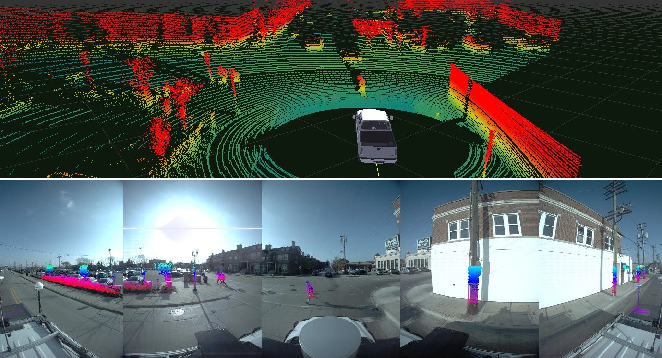
\includegraphics[scale=0.55]{figures/lidar-camera}
\caption[Lidar \& Camera view in self-driving cars]{Same environment, different modes (top: LIDAR view, bottom: camera view).}	
\label{fig:lidar-camera}
\end{figure}


%----------------------------------------------------------------------------------------
%	SECTION 
%----------------------------------------------------------------------------------------

\section{Proposed solution}\label{sec:proposed-solution}
In essence, the EMMA module is placed in front of and coupled with the deep learning model. The module multiplies each mode of the input sample by a weight so that the modes with the most useful features are amplified, while the modes that are unnecessary or contain too much perturbations are masked out. The amount of attention allocated to each mode is determined based on its importance, which is defined in terms of three intrinsically related properties, namely
\begin{itemize}
\item \textit{relevance}: the intrinsic informativeness of the mode for the predictive task at hand.
\item \textit{failure intensity}: the propensity of a mode to trigger undesirable activations in the neural network.\footnote{We suggest that a mode of the input sample that is significantly different from the training distribution may cause undesired activations in the neural network, thereby negatively affecting the predictions.}
\item \textit{coupling}: the interdependencies between the modes, which describe the extent to which the mode provide independent, complementary, redundant or conflicting information.
\end{itemize}
The module is designed in such a way that it is able to learn these three properties (and their interactions) for each mode. In other words, the module determines the attention to allocate to each mode on its general predictive power, the amount of perturbations it contains and the relationship it has with other modes. For example, this allows the module to mask out a specific failing mode provided that another mode can compensate for its failures. Let us stress that the determination of importance is done on a sample-per-sample basis.
\begin{figure}[!h]
\centering
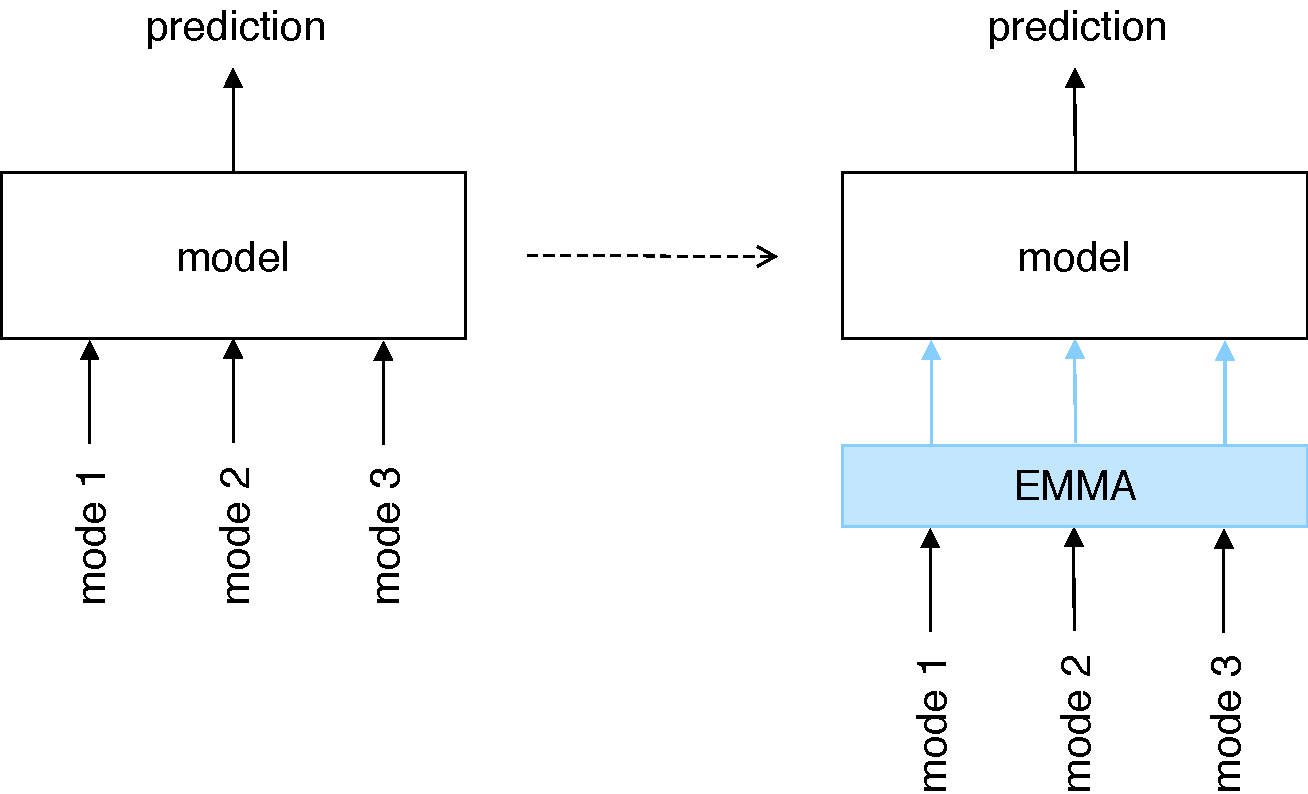
\includegraphics[scale=0.45]{figures/introduction-three-modes-with-emma}
\caption[Multi-Modal model with/without EMMA]{A multi-modal model with three input modes, without EMMA (left), augmented with EMMA (right).}	
\label{fig:main-idea}
\end{figure}

\subsection*{Software Implementation}
All the implemented models and experiments are available at \href{https://github.com/Werenne/energy-based-multimodal-attention}{this}\footnote{\url{https://github.com/Werenne/energy-based-multimodal-attention}} repository, with a wiki explaining how to run the experiments; \href{https://pytorch.org/}{PyTorch}\footnote{\url{https://pytorch.org/}} \citep{paszke} was the main framework used for the Machine Learning part.

%----------------------------------------------------------------------------------------
%	SECTION 
%----------------------------------------------------------------------------------------

\section{Contributions}
The contributions of this Master thesis can be summarised as follows
\begin{description}
\item \textbf{Contribution 1: an attention module improving the robustness against failing modes.} In Chapter \ref{chapter-emma}, the design of a new attention mechanism based on energy models \citep{ebm-tutorial} is discussed, that can be added to any multi-modal model. 
\item \textbf{Contribution 2: a simple yet powerful regularizer applying to attention mechanisms.} A common attention function is modified, establishing a link to the concept of capacity of psychology \citep{attention-is-effort}, which pertains to the amount of attention allocated among inputs. Subsequently, a new regularizer is introduced to control the capacity, whose purpose is to help generalise against unexpected situation.
\item \textbf{Contribution 3: a unified model for multi-modal attention.} In Chapter \ref{chapter-literature-review}, a review of the literature on attention in humans helps us identify how to construct a more complete multi-modal attention module.
\end{description}

%----------------------------------------------------------------------------------------
%	SECTION 
%----------------------------------------------------------------------------------------

\section{Thesis Outline}
The remainder of this work is organised as follows.
\begin{description}
\item \textbf{Chapter 2} explains the background (i.e. deep learning and energy models) this work is based upon.
\item \textbf{Chapter 3} reviews the literature on attention in psychology and deep learning, and the similarities between them.
\item \textbf{Chapter 4} describes a method for the estimation of the failure intensity of a mode.
\item \textbf{Chapter 5} presents the ideas behind the architecture of the Energy-based Multi-Modal Attention module (Contribution 1 \& 2).
\item \textbf{Chapter 6} presents an evaluation and analysis of the module outlined in Chapter \ref{chapter-emma} (Contribution 1 \& 2).
\item \textbf{Chapter 7} proposes a unified multi-modal attention module (Contribution 3).
\item \textbf{Chapter 8} concludes this work and suggests possible directions for future research.
\end{description}